% corrige espacamento de paginas pares que ficam diferente das impares
% devido a configuracao de impressao two-side da classe de documento
% remova o setlength abaixo caso queira retorar para a configuracao padrao:
%\setlength{\evensidemargin}{16pt}
\RequirePackage{helvet}
\renewcommand{\familydefault}{\sfdefault}
% ---
% Margens:
% esquerda 3cm direita 2cm
% topo 3cm base 2cm
\setlrmarginsandblock{3cm}{2cm}{*}
\setulmarginsandblock{3cm}{2cm}{*}
\checkandfixthelayout

% O tamanho do parágrafo é dado por:
\setlength{\parindent}{1.3cm}

% Controle do espaçamento entre um parágrafo e outro:
\setlength{\parskip}{0.2cm}  % tente também \onelineskip


\makeevenhead{plain}{}{}{\thepage}
\makeoddhead{plain}{}{}{\thepage}

\makeevenfoot{plain}{}{}{}
\makeoddfoot{plain}{}{}{}
% % caso queira que aparece nas referencias bibliograficas onde tais referencias
% % foram citadas, descomentar tambem o pacote \usepackage[brazilian,hyperpageref]{backref}
% % em pacotes.tex
% \renewcommand{\backrefpagesname}{Citado na(s) página(s):~}
% \renewcommand{\backref}{}
% \renewcommand*{\backrefalt}[4]{
% 	\ifcase #1 %
% 		Nenhuma citação no texto.%
% 	\or
% 		Citado na página #2.%
% 	\else
% 		Citado #1 vezes nas páginas #2.%
% 	\fi}%


\renewcommand{\imprimirdata}{%
    2019
}

\newcommand{\imprimircurso}{Bacharel em Sistemas de Informação}
%\newcommand{\curso}[1]{\def\imprimircurso{#1}}

\newcommand{\palavraChaveUm}[1]{\def\imprimirpalavrachaveum{#1}}
\newcommand{\palavraChaveDois}[1]{\def\imprimirpalavrachavedois{#1}}

\newcommand{\cdu}[1]{\def\nomecdu{#1}}
\newcommand{\dataDaAprovacao}[1]{\def\imprimirdatadaaprovacao{#1}}

\newcommand{\membroConvidadoUm}[1]{\def\imprimirmembroconvidadoum{#1}}
\newcommand{\membroConvidadoDois}[1]{\def\imprimirmembroconvidadodois{#1}}

\newcommand\BackgroundPic{%
	\put(0,0){%
		\parbox[b][\paperheight]{\paperwidth}{%
			\vfill
			\centering
			\includegraphics[width=\paperwidth,height=\paperheight,%
				keepaspectratio]{figuras/ifgformosa2015horizontal01}%
			\vfill
		}
	}
}

%\renewcommand{\imprimircapa}{%
%  \begin{capa}%
%    \center
%	\AddToShipoutPicture*{\BackgroundPic}
%
%%	\begin{huge}
%%		\textbf{\textsc{Trabalho de Conclusão de Curso}}
%%	\end{huge}
%
%    \vspace*{2.7in}
%	{\textbf{\large\imprimirinstituicao}}
%	\par
%	{\textbf{\large\imprimircurso}}
%
%	\vspace{0.5in}
%
%    {\ABNTEXchapterfont\bfseries\LARGE\imprimirtitulo}
%    \vspace*{\fill}
%    
%	\begin{flushright}
%    	\textbf{{\large{Autor: \imprimirautor}}}
%		\par
%    	\textbf{{\large{Orientador: \imprimirorientador}}}
%	\end{flushright}
%		
%    \vspace*{0.2in}
%    \textbf{{\large\imprimirlocal}}
%    \par
%    \textbf{{\large\imprimirdata}}
%    
%    \vspace*{2.2in}
%  \end{capa}
%}

\renewcommand{\imprimircapa}{%
	\begin{capa}%
		
		\vspace*{-2.2cm}
		\hspace*{-1cm}
		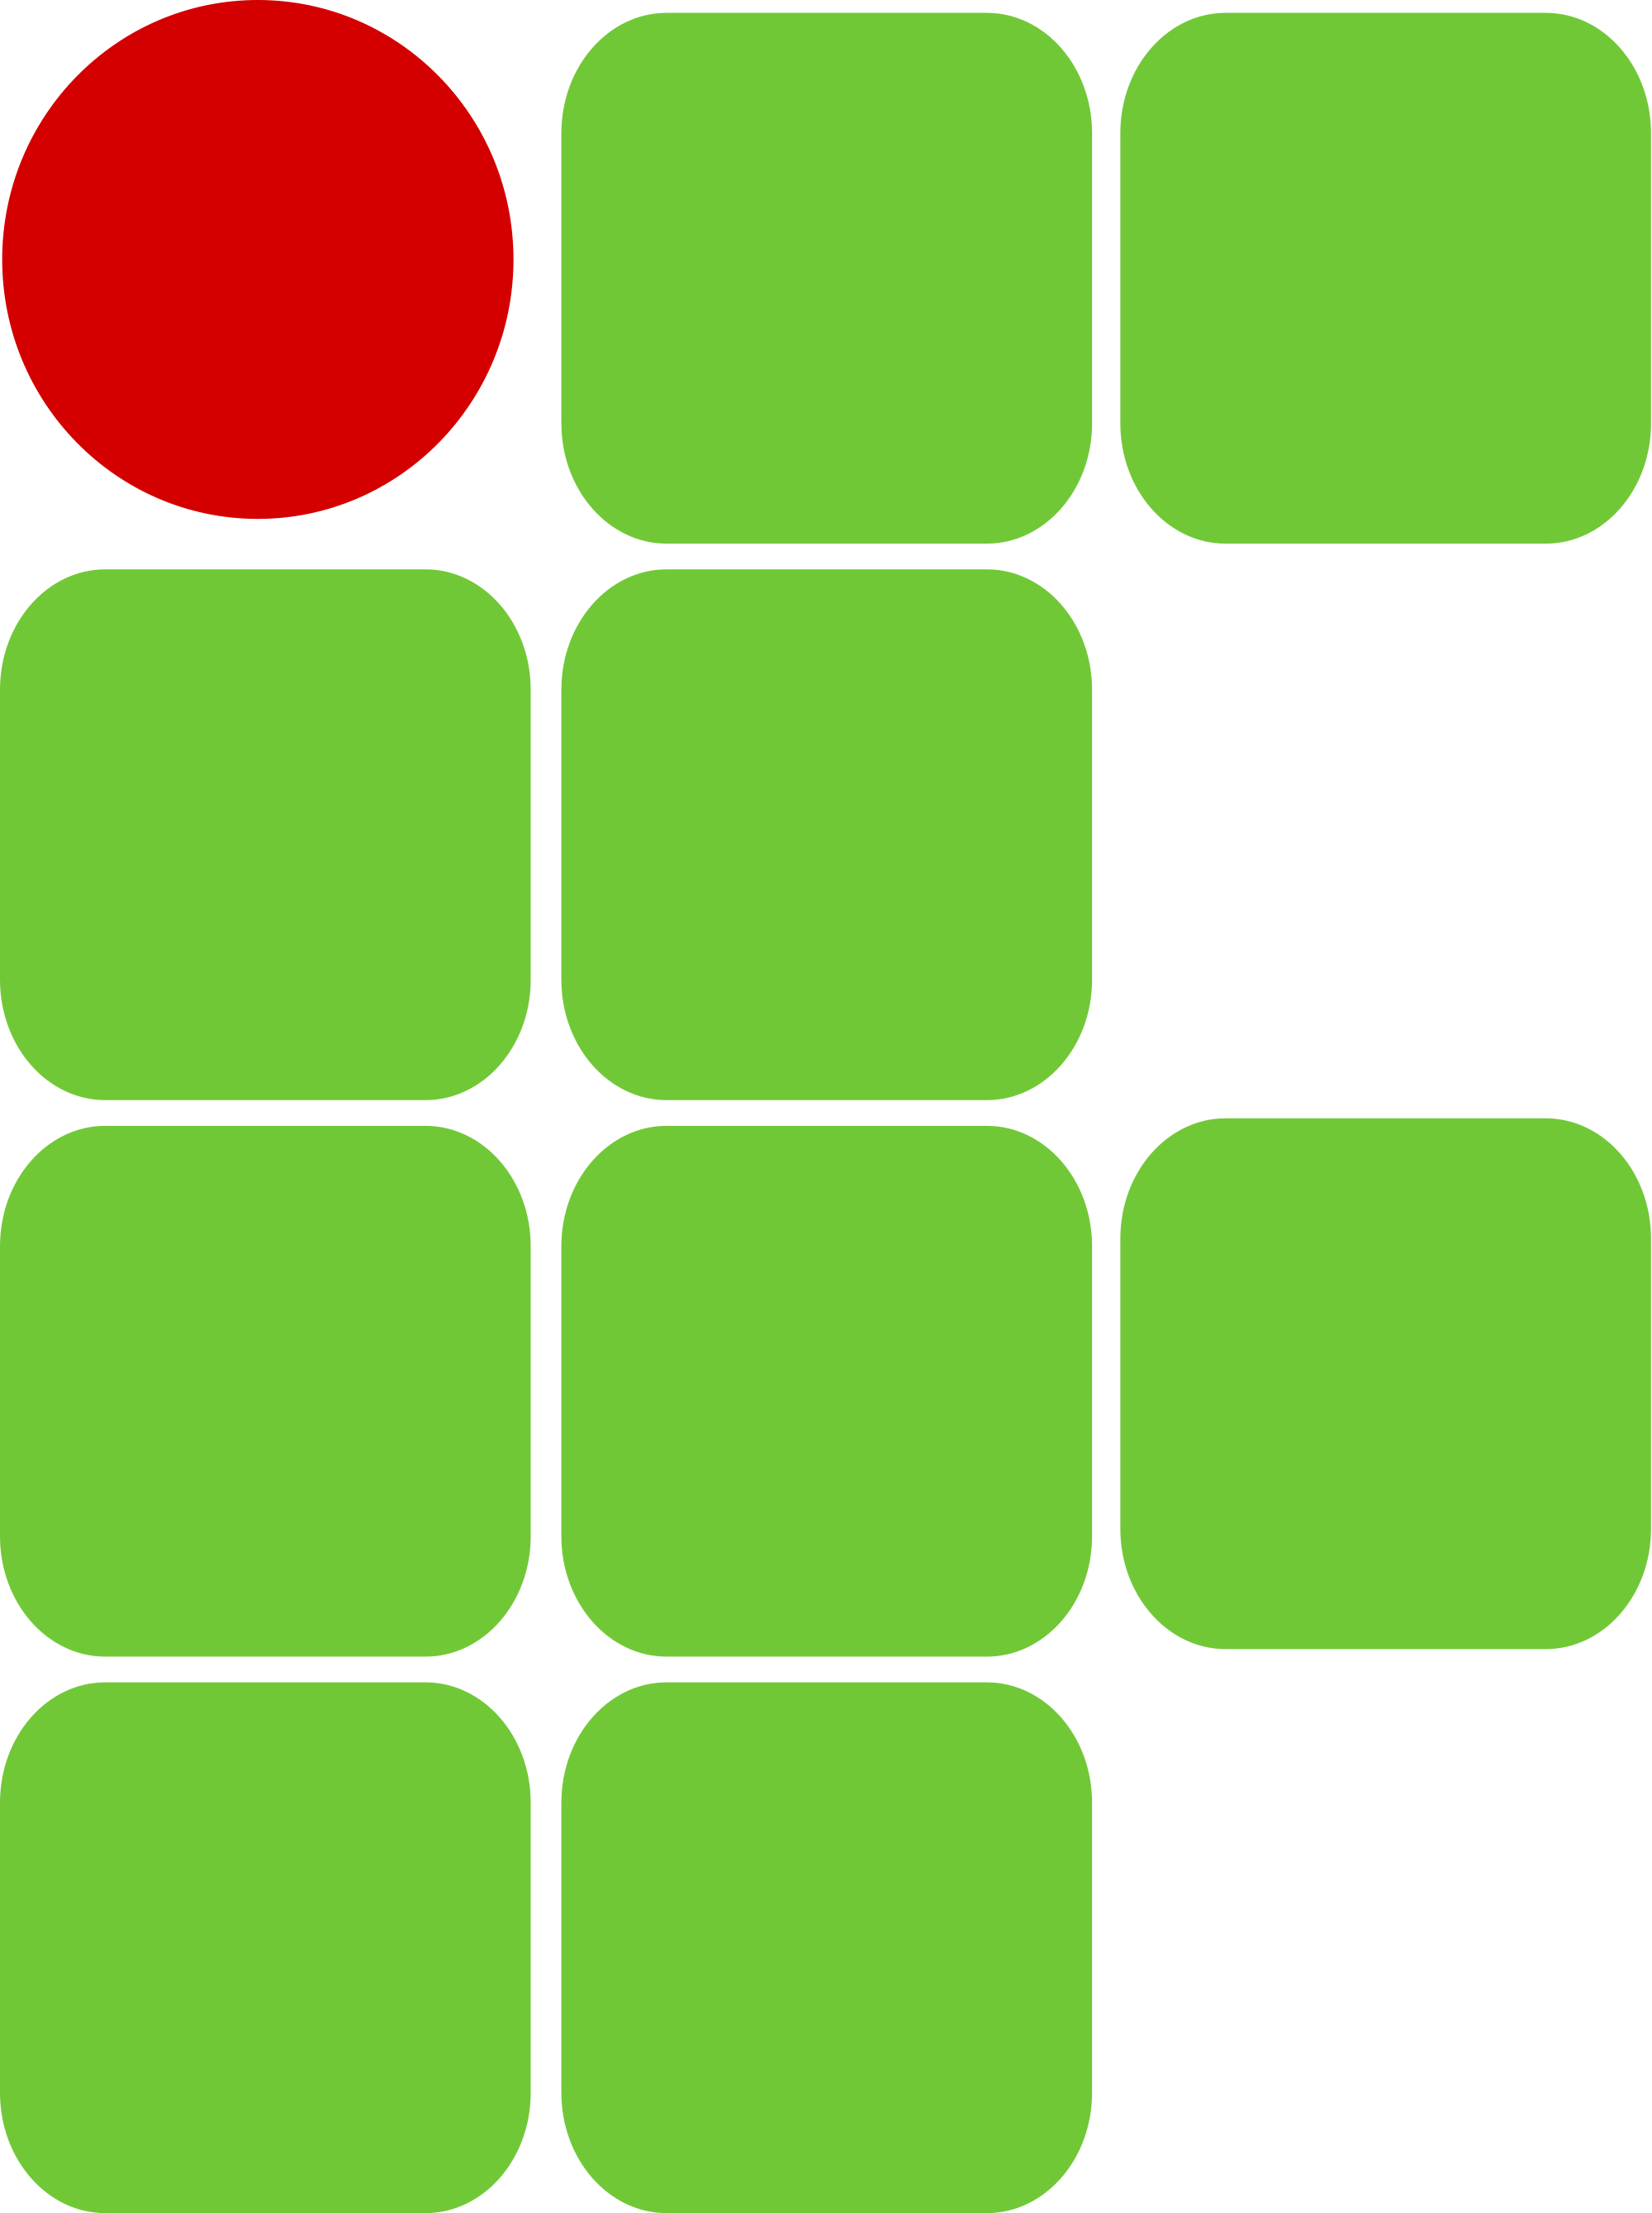
\includegraphics[width=1.5cm]{imagens/logo.png}
		\center
		\large INSTITUTO FEDERAL DO PARANÁ
		
		\vspace*{1cm}
		
		\MakeUppercase{\large\imprimirautor}
		
		\vfill
		\begin{center}
			\MakeUppercase{\large\bfseries\imprimirtitulo}
		\end{center}
		\vfill
		
		\MakeUppercase{\large\imprimirlocal}
		
		\large\imprimirdata
		
		\vspace*{1cm}
	\end{capa}
}

% os itens abaixo configuram a exibicao da lista de algoritmos
\renewcommand\lstlistingname{Algoritmo}
\renewcommand\lstlistlistingname{Lista de Algoritmos}
\let\oldlstlistoflistings\lstlistoflistings
\renewcommand{\lstlistoflistings}{%
  \begingroup%
  \let\oldnumberline\numberline%
  \renewcommand{\numberline}{\lstlistingname~\oldnumberline}%
  \oldlstlistoflistings%
  \endgroup}

% Configuração de fontes
\renewcommand{\ABNTEXchapterfont}{\bfseries}
\renewcommand{\ABNTEXchapterfontsize}{\normalsize}

\renewcommand{\ABNTEXpartfont}{\ABNTEXchapterfont}
\renewcommand{\ABNTEXpartfontsize}{\normalsize}

\renewcommand{\ABNTEXsectionfont}{\ABNTEXchapterfont}
\renewcommand{\ABNTEXsectionfontsize}{\normalsize}

\renewcommand{\ABNTEXsubsectionfont}{\sffamily}
\renewcommand{\ABNTEXsubsectionfontsize}{\normalsize}

\renewcommand{\ABNTEXsubsubsectionfont}{\sffamily}
\renewcommand{\ABNTEXsubsubsectionfontsize}{\normalsize}

\renewcommand{\ABNTEXsubsubsubsectionfont}{\sffamily}
\renewcommand{\ABNTEXsubsubsubsectionfontsize}{\normalsize}